% ============================================================
% Case Study and Results — Paper A (JNCA): the organizational case study,
% the cascade invariant, real-graph replication, rigor.
% All numbers are copied verbatim from the reproducibility package.
% ============================================================
\section{Case Study and Results}
\label{sec:results}

The \emph{case study} defines the organizational population, the communication graph with its rhythm, and the
cascade parameters that instantiate $G$, providing the concrete values for the symbols in
Sec.~\ref{sec:model}.

% ============================================================
\subsection{Case study: the organization and what is tested on it}
\label{sec:cs-setup}
The case study is a fully specified organizational ecosystem (Fig.~\ref{fig:casestudy}): $19$~firms from
distinct sectors (a bank, a hospital group, a software house, a law firm, a logistics company, an insurer,
a public office, \dots), each a small office of $\sim\!8$~accounts with one managing director, one senior
manager, and five to six specialists and analysts ($19$/$19$/$57$/$55$ accounts in the four seniority
levels). Everyone in a firm corresponds with everyone else in it, and the firms are tied into a ring of
business partnerships (director to director, plus one specialist counterpart per partnership), which gives
$N{=}150$ accounts and $556$ contact edges ($518$ inside firms, $38$ between partner firms). The population is
synthetic, but it is generated \emph{graph-first}: the organization graph is designed deterministically and
each persona is then generated \emph{in its node}, so that a persona's supervisor, coworkers, and external
contacts are \emph{real other personas} with real corporate addresses, and the graph closes internally. The
% ZMIANA: dodano opis budowy grafu Enron: bierzemy nagłówki Od/Do/Kopia i 2000
% najaktywniejszych kont (zostaje 1990). Wyjasniono tez roznice z artykulem B (818 nadawcow):
% tam potrzebny jest rytm kazdego nadawcy, wiec odrzucani sa nadawcy z mniej niz 25 mailami.
% Powod: bez tego 818 vs 1990 z tego samego korpusu wyglada na blad.
size $N{=}150$ is of the order of the core user set of the Enron corpus \citep{klimt2004enron}; the Enron
contacts graph used for validation (Sec.~\ref{sec:res-realgraphs}) is larger (${\approx}1970$~accounts), so the
real-graph replication also tests the mechanism at a larger scale; anomaly analysis of this corpus as a
communication graph has a long precedent, from scan statistics over Enron graphs \citep{priebe2005scan} onward. That graph is built from the
\texttt{From}/\texttt{To}/\texttt{Cc} headers of the maildir corpus as an undirected sender--recipient graph;
we keep the $2000$ highest-degree accounts and remove nodes left isolated by this filter, which leaves
${\approx}1970$~accounts. A companion study of the external-impersonation mode uses $818$~senders from the same corpus: its
multiplex requires a per-sender rhythm, so it keeps only senders with at least $25$~messages and a
non-empty active-bucket set; the difference is therefore a filter serving a different construction
(topology breadth here, per-sender temporal profiles there), not an inconsistency.

We divide the week into $T{=}28$ buckets (7~days $\times$ 4~six-hour blocks); an account's rhythm $\tau$ is the
set of its active buckets ($6$ per persona synthetically; on Enron derived from the \texttt{Date} headers).
Realistic noise: $15\%$ of legitimate mail arrives off-rhythm and $25\%$ of attacks mimic the rhythm. For the
cascade (Sec.~\ref{sec:m-detectors}) the per-contact infection probability is $p_\mathrm{inf}{=}0.6$ and the
maximum depth is $H{=}4$. Detector hyperparameters are fixed uniformly (Supplementary Tab.~S1).

\paragraph{What the case study tests} One kind of attack is injected into this graph, in three regimes
(Fig.~\ref{fig:casestudy}). A \emph{compromised internal account} $s_0$ mails its own contacts off-rhythm;
each recipient becomes a carrier with probability $p_\mathrm{inf}$, so the attack spreads as a cascade that
crosses into the partner firm through the business-partnership edge. The sender is a genuine contact
consistent with every static relation, so only the timing and the receiving-side wave give it away, and this
is what T1 must catch. Beyond the default cascade we probe three \emph{extreme} regimes, each chosen to stress
% przyczynowosc zdarzeniowa (liczniki widza wczesniejsze zdarzenia TEGO kubełka) blast
% jest znowu wygrana detektora wolumetrycznego (0.83 na SNAP, 0.63 na grafie case
% study) — i wlasnie dlatego reżim skryty jest tym, ktory go lamie: te same liczniki
% nie maja czego liczyc, gdy nosiciel wysyla raz na kubełek.
a specific claim rather than to represent typical traffic. \emph{(i)~Naive blast}: one carrier infects all
contacts at once, the maximally bursty case and the easy end of the scale---with event-causal counters the
volumetric detector \emph{does} catch it (AUC $0.83$ on the SNAP blast regimes, Tab.~\ref{tab:realgraphs}),
which is exactly what makes the stealthy regime the informative one.
\emph{(ii)~Stealthy spread} ($K$~carriers, one send per interval, down to $K{=}1$): the burst is smeared out,
so this is the case that \emph{breaks} volume detection and isolates the receiving-side signal.
\emph{(iii)~Single-recipient surgical attack} ($p_\mathrm{inf}{=}0$, fan-out~$1$): no propagation at all,
the \emph{blind spot} that no cascade detector can see, included to mark the lower boundary of the threat
model (T2). The stealthy-attacker and baseline contrasts are averaged over $20$ random seeds on synthetic
data and the detector hierarchy over $5$; real-graph validations use $8$ (Enron) and $3$ (SNAP) seeds.
Seed counts are stated in every caption.

\begin{figure}[pos=tbp]\centering
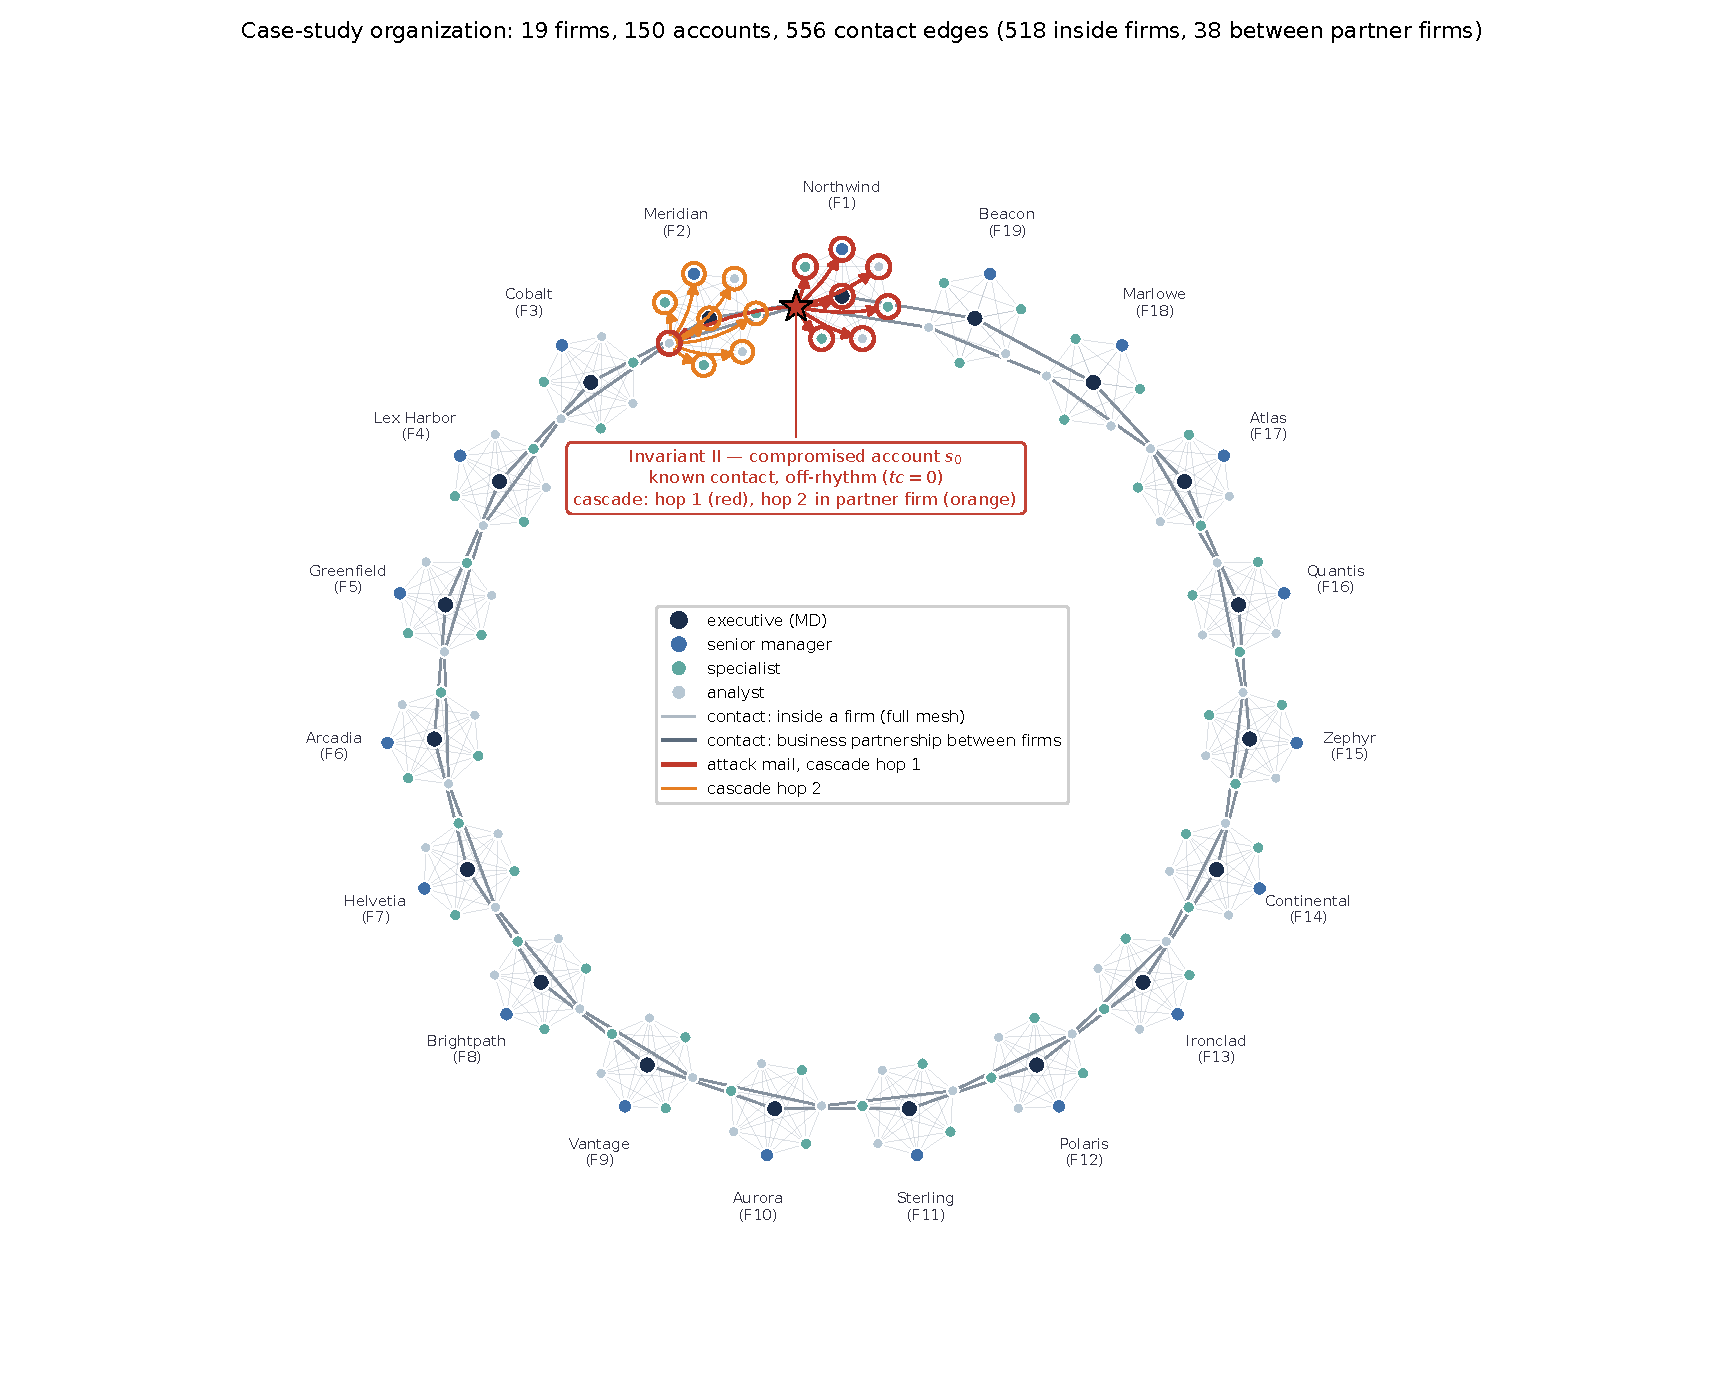
\includegraphics[width=\linewidth]{fig_org_case_study_cascade.pdf}
\caption[Case-study organization]{The case-study organization, drawn from the population data of the
reproducibility package: $19$~firms on a ring of business partnerships, $150$~accounts colored by seniority,
and the real contacts layer ($556$~edges). Overlaid is the attack the detectors must catch: a compromised
account $s_0$ (star) whose off-rhythm mail cascades through its own firm (hop~1, red) and into the partner
firm through the business-partnership edge (hop~2, orange). Every message in the cascade comes from a genuine
contact; only the timing and the receiving-side wave reveal it.}
\label{fig:casestudy}
\end{figure}

% ============================================================
\subsection{Results overview}
\label{sec:res-overview}
Table~\ref{tab:roadmap} maps the two research questions of Sec.~\ref{sec:intro} to the evidence; the
subsections follow that order. Results are reported on a victim or organization split, as AUC and, where
the operating point matters, sensitivity@FPR$1\%$; the time-shuffle control is applied to the detector
hierarchy on the case-study graph and on Enron. Seed counts are stated in each table or figure caption.

\begin{table}[pos=htbp]\centering\small
\begin{tabular}{@{}l p{0.29\linewidth} p{0.36\linewidth} p{0.22\linewidth}@{}}
\toprule
& \textbf{Sub-thesis} & \textbf{Main evidence} & \textbf{Verdict} \\
\midrule
RQ1 & the receiving-side cascade signal detects a compromise and stays above volume under a stealthy attacker (T1) &
Tabs.~\ref{tab:detectors}--\ref{tab:baselines}(a); real graphs: Tab.~\ref{tab:realgraphs};
Secs.~\ref{sec:res-detectors}--\ref{sec:res-baselines}, \ref{sec:res-realgraphs} &
stays above volume at every stealth level; vanishes under time shuffle; replicates in direction on three real graphs \\
\addlinespace
RQ2 & the signal needs fan-out~$\ge2$, degrades gracefully, and is a triage instrument at a real base rate (T2) &
Tab.~\ref{tab:baselines}(b); Supplementary Tabs.~S3--S4; Tab.~\ref{tab:baserate};
Secs.~\ref{sec:res-baselines}, \ref{sec:res-stability}, \ref{sec:res-rigor} &
fan-out~$\ge2$ needed; graceful under noise and scale; triage, not autonomous defense \\
\bottomrule
\end{tabular}
\caption{Map from research questions to evidence. Each verdict is established in the section listed.}
\label{tab:roadmap}
\end{table}

% ============================================================
\subsection{The cascade detectors}
\label{sec:res-detectors}
% ZMIANA: wszystkie liczby policzono od nowa po naprawie kodu. Dodano wiersz 'Library TGN'
% z brakujacymi liczbami (oficjalna implementacja z biblioteki PyG). Usunieto zdanie o
% 'AUC 0.49 detektora statycznego' — 0.49 to wynik innego eksperymentu (pelna slepota
% cech statycznych pod przejeciami kont), nie tej tabeli. Dodano zdanie, ze przewaga GNN
% nad kontekstem recznym dotyczy tylko zwyklej kaskady — w reżimie skrytym oba sa rowne.
A compromised account passes every static relation, so static graph position alone carries little
operational signal (the static GNN reaches AUC $0.76$ but only $0.039$ sensitivity at FPR~$1\%$). The
signal must therefore lie in the dynamics. Table~\ref{tab:detectors} tests T1 on the default cascade of
Fig.~\ref{fig:casestudy} and shows a clear hierarchy among detectors (bar chart in Supplementary Fig.~S1):
local 1-hop features are essentially useless (AUC $0.70$, sensitivity@FPR$1\%\!\approx\!0$), while a
hand-crafted multi-hop context reaches $0.81$. A static GNN captures the topology but misses the timing
($0.76$), and the volumetric baseline---evaluated in the same pass---ranks the naive cascade at $0.83$
but converts it into a worse operating point than the temporal model ($0.23$ vs $0.10$ sensitivity at
FPR~$1\%$), leaving the temporal GNN in the lead (AUC $0.87$, sensitivity@FPR$1\%$ $0.099$). This lead is
specific to the default cascade: under the stealthy regime of the second harness the temporal GNN and the
hand-crafted context are statistically indistinguishable (Sec.~\ref{sec:res-rigor}). This advantage is
temporal in the ablation sense. A simple time permutation drops the temporal GNN back to the static level
($0.87\!\to\!0.73$, sensitivity $0.099\!\to\!0.022$). Architecture choice matters less than the paradigm;
TGN-lite and TGAT-lite outperform the hand-crafted context ($0.87$ and $0.88$ vs $0.81$ AUC;
Supplementary Sec.~S1), and the library TGN
\citep{rossi2020temporal} reaches $0.79$ AUC with $0.112$ sensitivity@FPR$1\%$---below our TGN-lite on
AUC but close to it on the operational metric (the library-TGN row of Tab.~\ref{tab:detectors}, $3$~seeds).

\begin{table}[pos=tbp]\centering
\begin{tabular}{lcc}
\toprule
Detector & AUC & sensitivity@FPR$1\%$ \\
\midrule
\csname @@input\endcsname tables/tab_detectors 
\bottomrule
\end{tabular}
% ZMIANA: tabele generowane teraz bezposrednio z CSV (analysis/gen_tables.py) — nikt
% nie przepisuje liczb recznie. Dodano wiersz volumetric (COMPA) w tym samym przebiegu
% (A3) i wszystkie detektory dostaly jedna regule przyczynowosci zdarzeniowej (A1).
\caption{Cascade detectors on the case-study graph (victim split, $5$~seeds; library TGN row: $3$~seeds):
only the temporal models with node memory reach operational sensitivity ($0.099$ and $0.112$ at FPR~$1\%$),
the volumetric baseline ranks the naive cascade well ($0.83$) but converts it to a worse operating point
than the temporal GNN ($0.23$ vs $0.10$ at a much noisier threshold), and
shuffling the time order removes the temporal advantage ($\to\!0.73$), so the signal depends on temporal order.}
\label{tab:detectors}
\end{table}

% ============================================================
\subsection{The stealthy attacker}
\label{sec:res-stealth}
% ZMIANA: liczniki wolumetryczne przepisano na przyczynowosc na poziomie ZDARZENIA
% (patrza na wczesniejsze zdarzenia TEGO samego kubełka, nie tylko na wczesniejsze
% kubełki). Powod: recenzent zauwazyl, ze przy podziale na poziomie kubełka detektor
% wolumetryczny w ogole nie widzi rozwijajacego sie burstu — to czynilo go slomiana
% kuka, a to byloby zbyt latwe twierdzenie. Po naprawie volume widzi burst (w blast
% AUC 0.63; w harnessu SNAP nawet 0.83), ale w reżimie skrytym nadal nie ma z czego
% liczyc sygnalu: jedno wyslanie na kubełek zostawia puste KAZDE okno przyczynowe.
% Dodano wiersz 'rhythm-only' i udzialy poczty poza rytmem: ataki 75-79%,
% legalna 78-79% — sam bit rytmu nie odróżnia tu niczego. Liczby 15%/25% naleza do
% generatora artykulu B, nie tu.
Table~\ref{tab:stealth} is the headline test of T1: the stealthy attacker breaks volume, but not dynamics.
Against an attacker who evades detection by spreading its sends over time ($K$~carriers, one per interval),
the volume detector never develops a usable signal (AUC $0.50$--$0.63$ across all levels---its event-causal
counters now see the burst that builds up within a bucket, but one send per bucket leaves every causal
window empty), while the temporal GNN stays above it
at every level (AUC $0.59$, sensitivity@FPR$1\%$ $0.026$ vs $0.000$ for volume at $K{=}1$) because it
picks up the receiving side of the cascade.
% ZMIANA jezykowa: 'the volume detector breaks down ... while the temporal GNN degrades less' przepisano —
% powod: w liczbach absolutnych temporal traca WIECEJ niz volume (0.86->0.59 vs 0.63->0.50 od blast
% do K=1); prawdziwe twierdzenie brzmi 'temporal jest powyzej volume na kazdym poziomie K'.
Each detector is trained and tested within a single $K$~regime on a victim-disjoint split (Sec.~\ref{sec:m-detectors}),
so the volumetric weakness is not a train--test regime shift. We also report a rhythm-only control: in this
harness the off-rhythm share is nearly identical for attacks ($75$--$79\%$) and for legitimate traffic
($78$--$79\%$), because the benign buckets are drawn uniformly and the attack buckets consecutively, so the
rhythm bit alone stays at chance ($0.50$--$0.54$) and none of the signal can be attributed to it; the
$15\%/25\%$ rhythm parameters quoted in Sec.~\ref{sec:cs-setup} belong to the companion study's persona
generator, not to this harness. At $K{=}1$ the temporal signal is weak in absolute terms, and the hand-crafted context is
the strongest single detector ($0.73$, sensitivity $0.11$); the claim is the relative one---the receiving-side signal does not
collapse---which Table~\ref{tab:baselines} then qualifies. The temporal sensitivity
column is not monotone in $K$ ($0.026 \to 0.051 \to 0.042 \to 0.044$ from $K{=}1$ to $K{=}5$) while the corresponding AUC rises monotonically from
$K{=}2$ on ($0.74 \to 0.74 \to 0.76$); we attribute the non-monotonicity to seed-level variability of the low-FPR operating point,
which depends on a tail quantile of the score distribution, rather than to a change in mechanism.

\begin{table}[pos=tbp]\centering
% ZMIANA: dodano kolumne kontekstu recznego — powod: przy K=1 to on jest najlepszym detektorem
% (0.72 AUC, czulosc 0.097) i ukrywanie go w tekscie czynilo teze o GNN silniejsza niz dane.
\begin{tabular}{lcccccc}
\toprule
& \multicolumn{3}{c}{AUC} & \multicolumn{3}{c}{sensitivity@FPR$1\%$} \\
\cmidrule(lr){2-4}\cmidrule(lr){5-7}
Level & vol. & manual & temp. & vol. & manual & temp. \\
\midrule
\csname @@input\endcsname tables/tab_stealth 
\midrule
rhythm-only bit (all levels) & \multicolumn{3}{c}{$0.50$--$0.54$} & \multicolumn{3}{c}{$0.000$} \\
\bottomrule
\end{tabular}
% ZMIANA: liczby po przepisaniu wszytkich detektorow na przyczynowosc zdarzeniowa (A1)
% — pod atakiem skrytym (jedno wyslanie na kubelek) okna zdarzeniowe sa i tak puste,
% wiec kierunek bez zmian; kontekst reczny umocnil sie przy K=1 (czulosc 0.11).
\caption{Stealthy attacker on the case-study graph ($K$~carriers spread over time; $20$~seeds): the
volumetric detector is near chance at every level ($0.48$--$0.63$), the temporal GNN stays above it at
every level, and the hand-crafted context is the strongest detector at $K{=}1$ ($0.73$, sensitivity
$0.11$)---the headline result behind T1 is the receiving-side signal, read equally well by the learned
model and by the hand-crafted features, not the superiority of either. The
rhythm-only control stays at chance at every level, so the signal is the receiving-side wave, not the
rhythm bit.}
\label{tab:stealth}
\end{table}

Figure~\ref{fig:stealth} plots the same breakdown across $K$: both detectors weaken as the attack gets
stealthier, and the receiving-side signal keeps its margin over the volumetric one at every level.

\begin{figure}[pos=tbp]\centering
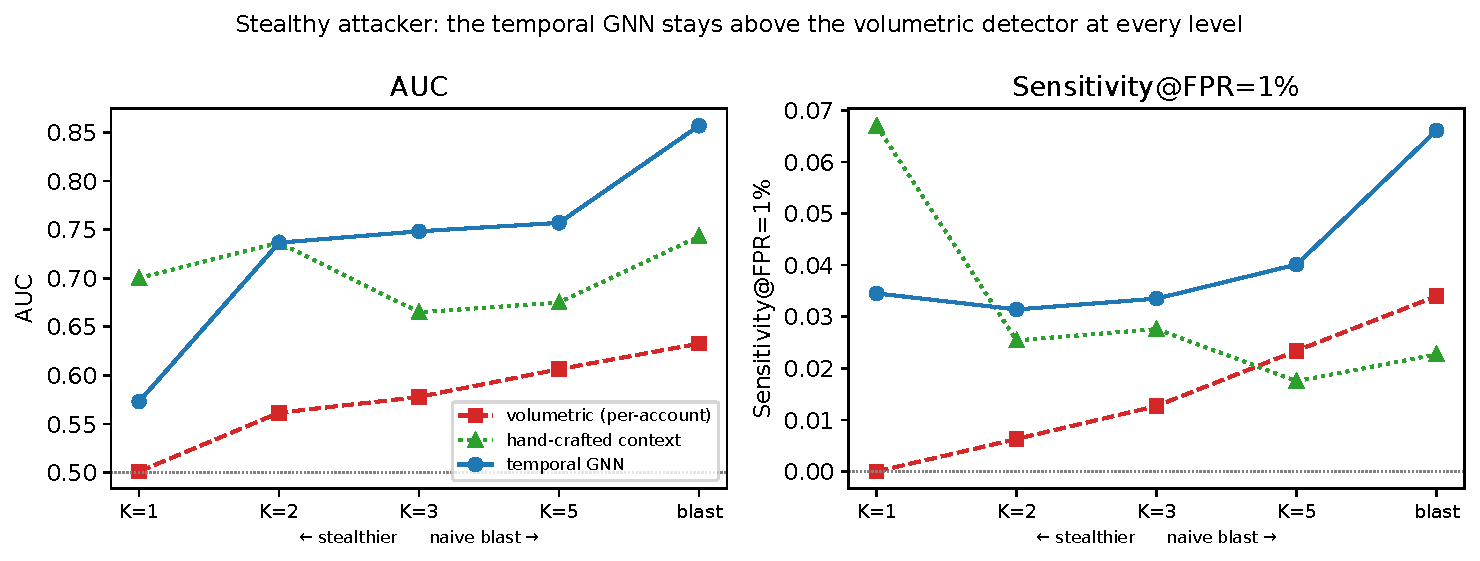
\includegraphics[width=\linewidth]{fig_cascade_stealth.pdf}
\caption[Stealth vs volume breakdown]{As the attack gets stealthier (smaller $K$) both detectors weaken,
but the temporal GNN keeps its margin over the volumetric one thanks to the cascade's receiving-side signal.}
\label{fig:stealth}
\end{figure}

% ============================================================
\subsection{Baselines and the boundary of the threat model}
\label{sec:res-baselines}
% ZMIANA: obie czesci tabeli wygenerowal na nowo odtworzony skrypt (oryginalnego
% brakowalo w paczce, wiec tabeli nie dalo sie odtworzyc; teraz 20 nasion losowosci).
% Dodano opis, czym roznia sie oba zestawy eksperymentow — bez tego to samo K dawalo
% rozne liczby i wygladalo to na blad. Wyjasniono tez wynik ~0.54 kontekstu recznego
% w ataku chirurgicznym: on liczy kontakte OFIARY trafione w przeszlych kubełkach,
% a atak jednokrotnie trafia wlasne kontakty nadawcy, wiec sasiedztwo ofiary
% nie jest odslane w oknie.
Table~\ref{tab:baselines} places this result against the two strong practical baselines and marks the boundary
of the threat model. This table comes from the second experiment harness (Supplementary Sec.~S6), so its
$K{=}1$ values differ slightly from Tab.~\ref{tab:stealth}. In the stealthy regime (block~a) the
path-based detector and the hand-crafted context lead under extreme stealth ($K{=}1$: $0.74$ and $0.77$,
ahead of the temporal GNN $0.63$) but degrade with reach (path $0.74\!\to\!0.65$), while the temporal GNN
has the largest end-to-end gain ($0.63\!\to\!0.85$) and leads from $K{=}3$ on. The two harnesses
differ in the generator and the population, not in the feature definitions: Tab.~\ref{tab:stealth} uses the
$150$-account case-study graph with consecutive-bucket stealth and uniform benign buckets, while
Tab.~\ref{tab:baselines} uses a $600$-account synthetic organization with an $8$-bucket send spacing,
$30\%$ rhythm mimicry, and $15\%$ off-rhythm benign traffic, plus a benign matched to the attack
(Sec.~\ref{sec:m-detectors}). Two remarks on reading this table. First, the path-based baseline keeps its
score although the look-ahead is removed: the corrected momentum counts \emph{past} targets---a different
signal, not a subset of the uncorrected one---and the harness uses its own generator, whose benign
protocol ($15\%$ off-rhythm, spread $8$, mimicry $0.3$) differs from the first harness, so part of the
difference against the stealth table is a harness difference, not only the causal fix. Second, the $K{=}1$ row has no
single winner among path-based and hand-crafted detectors ($0.74$ vs $0.77$); neither should be read as
the regime's best detector without per-seed intervals. The ablation column ``path (no precursor)''
answers the question of how much of the path baseline's stealth performance is carried by its precursor
feature, which largely coincides with the freshness bit of the hand-crafted context: zeroing it out
drops the path baseline by $0.06$--$0.12$ AUC at every stealth level ($0.74\!\to\!0.62$ at $K{=}1$,
$0.82\!\to\!0.79$ at blast) but leaves the surgical regime untouched ($\approx\!0.50$, where the feature is
already uninformative), so the precursor is the path baseline's stealth signal, not its surgical one.

In the surgical regime (block~b, no propagation at all, $p_\mathrm{inf}{=}0$) a single-recipient
attack is undetectable by every detector (AUC $0.48$--$0.53$): the signal requires fan-out~$\ge2$, and this is
the measured lower boundary of what the detectors can see (T2). Block~(b) also shows that propagation itself
is not required: with $p_\mathrm{inf}{=}0$ and fan-out~$\ge2$ the attack is caught by the volume detector
($0.68$--$0.83$) and by the temporal GNN ($0.75$--$0.94$), because several recipients in one neighborhood hit
at once already form a synchronized sending burst and a receiving-side wave. What the signal needs is
fan-out, not a cascade; the cascade matters because it is what lets a stealthy attacker reach many victims
\emph{without} such a burst. In this regime the hand-crafted context is structurally near-blind
($\approx\!0.55$ at every fan-out): its burst feature counts the \emph{victim's} contacts hit in strictly
past buckets, but a surgical carrier hits each of its own contacts once at staggered buckets, so a victim's
neighborhood is not revisited within the window; the volume detector sees the carrier's own multi-send
pattern and the temporal memory accumulates the staggered sends.

\smallskip\noindent\textbf{Legal broadcast waves as hard negatives.} A cascade detector that fires on
\emph{any} wave would be useless in practice, because real organizations contain legal broadcast waves
(newsletters, HR announcements, incident communications). We inject two classes of them
($20$~seeds; \texttt{exp\_legal\_cascade.csv}). \emph{Easy waves}: contact-preserving, in-rhythm, fan-out~$2$,
$30\%$ of the attack volume. \emph{Hard waves}: deliberately off-rhythm, fan-out~$6$, three hops through
the contact graph including the inter-firm partnership edges---structurally as wave-like as the attack, and
differing only in intent. Both cost almost nothing in the default cascade: volume moves $0.834\!\to\!0.830$
(easy) $\to\!0.817$ (hard), hand-crafted $0.805\!\to\!0.801\!\to\!0.792$, temporal $0.868\!\to\!0.870\!\to\!0.879$---the
learned model is \emph{more} accurate with the extra negatives to learn from. Under the stealthy attack the
same holds with the hard waves present: temporal $0.746$ vs volume $0.534$ and hand-crafted $0.653$. The
legal waves are sender-initiated and paced like the background, so they look exactly like what the
receiving-side features expect of legitimate traffic; the contrast with the stealthy \emph{attack}---which
hits the same contact pattern but paces its sends to hide the burst---comes from timing, not topology. The
measured boundary of the threat model is therefore two-sided: the detectors do not need a malicious cascade
to fire, but they also do not fire on a merely synchronized legal one, even off-rhythm and multi-hop.

\begin{table}[pos=tbp]\centering
\begin{tabular}{lccccc}
\toprule
Regime / level & vol. & path & path (no precursor) & manual & temp. \\
\midrule
\multicolumn{6}{@{}l}{\emph{(a) Stealthy cascade: $K$ carriers, one send per bucket, $p_\mathrm{inf}{=}0.6$ (reach in parentheses)}} \\
\csname @@input\endcsname tables/tab_baselines 
\bottomrule
\end{tabular}
% ZMIANA: po A1 wszystkie detektory maja przyczynowosc zdarzeniowa; kontekst reczny
% i hopper widza teraz fale w kubełku — hopper umocnil sie pod blast (0.82), a
% ablacja hopper-bez-precursor pokazuje udzial cechy precursor.
\caption{Baselines and the boundary of the threat model (AUC, $20$~seeds; path-based baseline in the spirit of
Hopper \citep{ho2021hopper}; ``path (no precursor)'' zeroes the precursor feature of the path baseline).
(a)~Under a stealthy cascade the path-based detector and the hand-crafted
context lead only at $K{=}1$, the path-based detector degrades with reach, and the temporal GNN
has the largest end-to-end gain, leading from $K{=}3$ on; removing the precursor costs the path baseline
$0.06$--$0.12$ AUC at every level. (b)~With no
propagation, a single-recipient attack is invisible to every detector ($0.48$--$0.53$); the signal needs
fan-out~$\ge2$. The two blocks are not comparable at ``1'': in (a) $K{=}1$ still propagates, in (b) fan-out~$1$
is a surgical attack with no cascade at all.}
\label{tab:baselines}
\end{table}

% ============================================================
\subsection{Stability and inductive generalization}
\label{sec:res-stability}
% ZMIANA: dodano wyjasnienie dziwnego wyniku: im mniejsze prawdopodobienstwo zarazenia,
% tym lepsza detekcja (0.97 przy 0.05). Powod: ruch legalny jest staly, a liczba maili
% ataku rosnie z p_inf — przy malej wartosci ataki to niemal same pojedyncze wybuchy,
% rzadka i latwa do odróżnienia klasa. Liczby w S3 policzono od nowa.
Two checks bound the reading of T1. The cascade model sweep (Supplementary Tab.~S2) shows the hierarchy
holding across the whole range $p_\mathrm{inf}\!\in\![0.05,0.9]$ and depth; the receiving-side signal does not
vanish at a realistically low $p_\mathrm{inf}$ (temporal GNN $0.84$--$0.97$ across the sweep, with the
volumetric baseline a solid mid-table $0.82$--$0.88$). The temporal AUC is highest at
the lowest $p_\mathrm{inf}$ ($0.97$ at $0.05$) because the class composition changes along the sweep: the
benign volume is fixed, while the number of attack events grows with $p_\mathrm{inf}$ (more infections mean
more carriers and more sends), so at a low $p_\mathrm{inf}$ the attack class is small and concentrated in
patient-zero bursts that are nearly separable, and it grows more benign-like as propagation strengthens.
Under inductive validation across disjoint organizations (Supplementary Tab.~S3 and Fig.~S2), the temporal
GNN does \emph{not} lead on AUC---it is behind the hand-crafted context at every scale ($0.72$ vs $0.79$ at
$19$~organizations, $0.70$/$0.73$ vs $0.77$/$0.82$ at $30$ and $200$) and, with the volumetric baseline
included in the same pass, volume leads the inductive setting outright: $0.83$--$0.85$ AUC and
sensitivity@FPR$1\%$ of $0.24$--$0.33$, against $0.09$ for the temporal GNN at $19$~organizations.
% ZMIANA (A3, recenzja wewnetrzna r2): dodanie volume do przebiegu indukcyjnego OBALO
% przewage operacyjna temporalu w tym ustawieniu — volume generalizuje na niewidziane
% firmy lepiej (cechy per-nadawca nie zaleza od topologii), sygnal odbiorczy jest
% topologo-zalezny. Uczciwie zawezamy: T1 wygrywa in-distribution i pod stealth,
% volume wygrywa transfer miedzy organizacjami. Temporal zachowuje przewage nad
% kontekstem recznym (1.8-2.3x czulosc), ale nie nad volume.
The honest reading is that T1's inductive boundary is here: the receiving-side wave wins in-distribution
and under the stealthy attacker, but its per-sender deviation features make the volumetric detector the
best \emph{transfer} detector to organizations never seen in training, while the temporal GNN still holds
a $1.8$--$2.3\times$ operational edge over the hand-crafted context at every scale.

\noindent Cascade dynamics thus overcome the blindness of static relations to a compromise and, unlike the
volume detector, do not collapse under a stealthy attacker; the advantage depends on temporal order, but it
does not transfer across organizations as well as the volumetric signal does. The next question is whether the mechanism is a property of the generator or of communication
graphs.

% ============================================================
\subsection{Validation on real communication graphs}
\label{sec:res-realgraphs}
% ZMIANA: liczby policzono od nowa po przepisaniu licznikow wolumetrycznych na
% przyczynowosc zdarzeniowa (patrza tez na wczesniejsze zdarzenia TEGO kubełka).
% Skutek na SNAP: detektor wolumetryczny widzi teraz rozwijajacy sie burst i wygrywa
% naiwny blast (0.83) — jego stara porazka w blast byla artefaktem okien kubełkowych.
% W reżimie skrytym nadal pada (0.59-0.64), a kontekst reczny i temporalny wygrywaja
% (0.78-0.86). Obserwacja 'temporal lepszy pod stealth niz blast' pozostaje i ma teraz
% wyjasnienie: na rzadkim SNAP-owym grafie wszystkie wyslania nosiciela w blast siedza
% w jednym kubełku, wiec okna scisle przeszłe zdarzen hop-1 sa puste — to samo dotyczy
% kontekstu recznego (0.63 w blast vs 0.86 stealth), co potwierdza wyjasnienie.
Real graphs (Enron, two SNAP graphs) are used to validate the mechanism where the structure and rhythms are
real. The qualitative hierarchy of methods established on one topology must carry over to another, in line
with the definition of effectiveness (Sec.~\ref{sec:effectiveness}). The attack labels are controlled
injections under a matched design, so legitimate traffic and attack are edges with the same distribution of
endpoints and degrees, distinguished only by their temporal pattern.

Table~\ref{tab:realgraphs} reports both replications, with the volumetric detector evaluated on all
three real graphs. On the real Enron contacts graph (${\approx}1970$~accounts,
$8$~seeds, leak-free; block~a) the regime contrast is the same as on the SNAP graphs: under the naive
blast the volumetric detector wins ($0.87$, sensitivity $0.22$)---its event-causal counters see the
synchronized burst building up within a bucket---with the receiving-side hierarchy behind it (hand-crafted
context $0.77$, temporal GNN $0.81$; bar chart in Supplementary Fig.~S4) and the time shuffle leveling the
temporal detector toward the hand-crafted result ($0.75$). Under the stealthy attacker the picture flips:
the hand-crafted context reaches $0.89$ (sensitivity $0.27$) and the temporal GNN $0.84$ ($0.16$), while
volume stays at $0.67$ and the 1-hop baseline at $0.59$; the shuffle control costs the temporal detector
$0.10$~AUC, so the advantage depends on temporal order here as well. On \texttt{email-Eu-core}
\citep{paranjape2017motifs} and \texttt{CollegeMsg} \citep{panzarasa2009patterns} (\citep{leskovec2014snap};
block~b, bar chart in Supplementary Fig.~S3) the same contrast replicates: under the stealthy attacker the
hand-crafted context reaches $0.84$/$0.82$ and the temporal GNN $0.79$/$0.83$, while the volumetric detector
stays at $0.62$--$0.63$ (the better receiving-side detector is $+0.16$/$+0.20$ AUC ahead); under the naive
blast the volumetric detector wins on both graphs ($0.83$) while the receiving-side detectors drop to
$0.61$--$0.65$. The blast inversion has a structural explanation that the two methods share: in the real-graph
blast all sends of a carrier share one bucket, so the past windows of hop-1 events are empty and the
receiving-side wave leaves no readable trace there, whereas on the dense case-study cliques the same burst
stays visible through the contacts feature; under the stealthy cascade the staggered buckets feed the memory.
The predictivity probe is therefore positive in the regime-level sense of
Sec.~\ref{sec:eval}: on each of the three real graphs the stealthy regime puts the receiving-side detectors
ahead of volume exactly where the attacker hides, and the blast is volume's best case everywhere. With
$3$--$8$ seeds per graph a per-graph Wilcoxon test cannot reach conventional significance (the minimum
two-sided $p$ is $0.25$ for $n{=}3$), so we report the real-graph replications as directional confirmations,
not as significance tests. One caveat we quantify in Sec.~\ref{sec:res-rigor}: part of the receiving-side
margin in the stealthy regime rides on the \emph{injected-attack timing signature}---the deterministic
send gaps of the injected events differ from the background's timing---so we repeat the stealthy regime
with attack times drawn from the background's empirical gap distribution; the receiving-side signal
survives in the learned temporal model, but not in the hand-crafted features. The practical takeaway of
the real-graph block is therefore not ``volume never works'' but ``volume fails exactly in the stealthy
regime, which is the threat model this paper is about---and even there, only the learned memory reads the
wave once the injection signature is removed.''

\begin{table}[pos=tbp]\centering
\begin{tabular}{llcc}
\toprule
Graph (regime) & Detector & AUC & sensitivity@FPR$1\%$ \\
\midrule
\multicolumn{4}{@{}l}{\emph{(a) Enron contacts graph, ${\approx}1970$~accounts, matched design, $8$~seeds}} \\
\csname @@input\endcsname tables/tab_realgraphs
\bottomrule
\end{tabular}
% ZMIANA: A5 — dodano detektor wolumetryczny na Enronie w obu rezymach; A1 — jedna
% regula przyczynowosci. Na WSZYSTKICH trzech realnych grafach ten sam kontrast rezymow:
% blast wygrywa volume (0.83-0.87 — widzi burst), stealth wygrywa sygnal odbiorczy
% (0.84-0.89 vs 0.62-0.67). Uwaga A2: pod stealth czesc przewagi to sygnatura czasow
% iniekcji — patrz kontrola w sekcji Rigor (mini-tabela): po wylosowaniu czasow ataku
% z rozkladu tla kontekst reczny spada ponizej volume, temporal trzyma 0.70-0.76.
\caption{Replication on three real communication graphs, with the volumetric detector on all
three (AUC / sensitivity@FPR$1\%$). (a)~On Enron, under the naive blast the volumetric detector wins
($0.87$) and the case-study hierarchy follows behind it; under the stealthy attacker the receiving-side
signal wins ($0.89$ hand-crafted context, $0.84$ temporal GNN vs $0.67$ for volume), with the time
shuffle costing the temporal detector $0.10$ AUC. (b)~The same regime contrast replicates on both SNAP
graphs: volume wins the blast ($0.83$), the receiving-side detectors win the stealthy regime
($0.82$--$0.84$ vs $0.62$--$0.63$). The stealthy-regime numbers embed the injected-attack timing
signature quantified in Sec.~\ref{sec:res-rigor} (injection control).}
\label{tab:realgraphs}
\end{table}

% ============================================================
\subsection{Rigor: what it means for a detector to work}
\label{sec:res-rigor}
% ZMIANA: testy porownawcze policzono od nowa po przepisaniu licznikow COMPA na
% przyczynowosc zdarzeniowa. Nowy wynik: sygnal odbiorczy bije volume z duzym zapasem
% (+0.104, p<0.001, delta 0.96), a GNN vs kontekst reczny to -0.008 przy p=0.39 —
% statystycznie zero roznicy w OBU protokolach benign (w harnessu baselines +0.019),
% wiec wniosek o nierozroznialnosci jest silniejszy niz przed naprawa. Badanie szumu
% etykiet zostalo przy reżimie K=3. Arytmetyka bazowa: czulosc r=0.12; ~830 fałszywych
% alarmow na wykryty atak przy czestosci 1:10^4; w reżimie skrytym r=0.03 -> ~3300.
The results follow the definition of effectiveness (Sec.~\ref{sec:effectiveness}) and the operational limits are
marked, so the headline numbers read as a lower bound rather than a deployment claim.

\smallskip\noindent\textbf{Variance and significance.} The stealthy-attacker, baseline, and label-noise
contrasts are averaged over $20$ seeds on synthetic data; the detector hierarchy (Tab.~\ref{tab:detectors})
uses $5$, the cascade sweep (Supplementary Tab.~S2) $8$, the inductive validation (Supplementary Tab.~S3)
$5$ or $3$, the sensitivity--FPR curve (Supplementary Fig.~S5) $10$, and the real-graph replications
(Tab.~\ref{tab:realgraphs}) $8$ (Enron) and $3$ (SNAP); aggregate values for every table are
available in the reproducibility package (\texttt{code/results/*.csv}), and per-seed values are dumped
as \texttt{*\_perseed.csv} files by every headline script (bootstrap $95\%$~CIs in
\texttt{code/results/ci/}). Strengthening the main contrast on
$20$~seeds at the stealthy point of the second harness ($K{=}2$, spread~$8$, mimicry~$0.3$;
Sec.~\ref{sec:res-baselines}) with a paired Wilcoxon test and Cliff's~$\delta$, the receiving-side signal
beats the volume detector significantly and with a large effect (temporal GNN $+0.115$ AUC over COMPA,
$p<0.001$, $\delta{=}0.98$), the hand-crafted context beats it as well ($+0.095$, $p<0.001$,
$\delta{=}0.91$), while the temporal GNN and the hand-crafted context are statistically indistinguishable
at this point ($+0.021$, $p{=}0.19$, $\delta{=}0.26$). We also repeated the contrast under the benign
protocol of Tab.~\ref{tab:baselines} ($15\%$ off-rhythm traffic): the margins are stable there
($+0.109$ over COMPA, $p<0.001$; temporal vs manual $+0.027$, $p{=}0.04$), so under off-rhythm benign
traffic the learned model gains a small but nominally significant edge over the hand-crafted
features---the honest reading is that the two receivership detectors are near-equivalent, with the balance
tipped slightly toward the learned model when the background is noisier. Under a stealthy attack, then, it is the
receiving-side signal---read equally well by the learned temporal model and by the hand-crafted
features---that surpasses volume detection. For the whole curve, instead of a single threshold we report the
sensitivity--FPR curve (Supplementary Fig.~S5): at a realistically low FPR ($0.1\%$) the sensitivities fall to
$0.005$--$0.040$ in the blast regime and $0.001$--$0.023$ in the stealthy regime.

\smallskip\noindent\textbf{The volumetric weakness is structural, not a tuning artifact.} The volumetric baseline has no
window or threshold to tune: its three features are counts over the observed stream (recipient novelty, time
novelty, sender activity; Supplementary Sec.~S6) fed to the same learner as every other tabular detector.
Its counters are event-causal---an event's features may use earlier events of the same bucket, so a burst
that builds up within a bucket \emph{is} visible to it (this is why it wins the naive blast on the SNAP
graphs, Tab.~\ref{tab:realgraphs}). Its weakness under the stealthy attacker is therefore a property of the
attack model---one send per bucket per carrier leaves every causal window without a surge to
see---rather than of a baseline configuration.

\smallskip\noindent\textbf{The injected-attack timing signature, and what survives its removal.}
% ZMIANA (A2, recenzja wewnetrzna r2): nowa kontrola sygnatury iniekcji. Powod: na
% realnych grafach reżim stealth wygladal LATWIEJSZY niz blast (kontekst reczny 0.89 na
% Enronie), co budzilo podejrzenie, ze detektory czytaja artefakt czasow wstrzyknietych
% zdarzen (deterministyczne odstepy 1 kubelek), nie fale odbiorcza. Trzy narzedzia: test KS
% odstepow atak vs tlo, czysto czasowa sonda (odstepy/regularnosc wysylek nadawcy), i
% wariant 'stealth-empirical' z czasami ataku losowanymi z rozkladu tla. Sygnature
% POTWIERDZONO (KS 0.46-0.79); po jej usunieciu sygnal odbiorczy trzyma TYLKO nauczony
% model (temporal 0.69-0.76 > volume 0.57-0.67), a cechy reczne spadaja do poziomu volume
% (0.60-0.64). To zaweza twierdzenie T1 na realnych grafach do modelu nauczonego.
The stealthy regimes of Tab.~\ref{tab:realgraphs} use injected attack events, and injected times can carry
an artifact: the sends of a stealthy carrier arrive at deterministic, evenly spaced gaps that the
background traffic never produces. A two-sample KS test confirms the signature on all three real graphs
(statistics $0.46$--$0.79$, $p\!<\!10^{-43}$), and a purely temporal probe---a LightGBM over nothing but
inter-send gaps, their regularity, and sender activity, with no graph feature at all---reaches AUC
$0.71$--$0.76$ under the stealthy regime: much of the apparent margin rides on \emph{when} the injections
happen, not on the receiving-side wave. Tab.~\ref{tab:injection} therefore repeats the stealthy regime with
the attack send times drawn from the background's empirical gap distribution (\emph{empirical} rows): the
KS distance collapses to $0.04$ ($p\approx0.5$), the probe to $0.54$--$0.63$, and the hierarchy changes---
the learned temporal GNN keeps a margin over volume on all three graphs ($0.69$--$0.76$ vs
$0.57$--$0.67$), while the hand-crafted features fall back to the volumetric level
($0.60$--$0.64$). The honest claim of T1 on real graphs is thus narrower than the raw table suggests: the
receiving-side signal survives an attack that paces like the background, but only the learned memory
reads it; the hand-crafted context was reading the injection.

\begin{table}[pos=tbp]\centering\small
\begin{tabular}{llccccc}
\toprule
Graph & Timing & KS & probe & vol. & manual & temp. \\
\midrule
\multirow{2}{*}{Enron} & injected & $0.79$ & $0.76$ & $0.69$ & $\mathbf{0.88}$ & $0.86$ \\
 & empirical & $0.04$ & $0.63$ & $0.67$ & $0.64$ & $\mathbf{0.76}$ \\
\multirow{2}{*}{\texttt{email-Eu-core}} & injected & $0.77$ & $0.71$ & $0.64$ & $\mathbf{0.85}$ & $0.83$ \\
 & empirical & $0.08$ & $0.54$ & $0.60$ & $0.60$ & $\mathbf{0.70}$ \\
\multirow{2}{*}{\texttt{CollegeMsg}} & injected & $0.69$ & $0.70$ & $0.62$ & $\mathbf{0.82}$ & $0.77$ \\
 & empirical & $0.04$ & $0.56$ & $0.57$ & $0.61$ & $\mathbf{0.69}$ \\
\bottomrule
\end{tabular}
\caption{Injection-signature control (stealthy regime, $3$~seeds; \texttt{exp\_injection\_probe.csv}). KS:
two-sample statistic of inter-send gap distributions, attack vs background. Probe: AUC of a purely
temporal detector (no graph features). ``Empirical'' rows re-run the regime with attack times drawn from
the background's empirical gap distribution. The receiving-side margin over volume survives the
signature's removal only in the learned temporal GNN (bold), not in the hand-crafted features.}
\label{tab:injection}
\end{table}

\smallskip\noindent\textbf{Label noise.} Flipping an increasing fraction of training labels (Supplementary
Tab.~S4) shows that the learned GNN degrades fastest (temporal $0.72\!\to\!0.59$ at $20\%$ noise, volume only
$0.60\!\to\!0.57$, hand-crafted $0.66\!\to\!0.61$). Under realistic label noise the advantage of the learned model shrinks---another boundary
of T2.

\smallskip\noindent\textbf{Base rate.} Sensitivity at a given FPR is independent of prevalence, but
precision drops when the attack is rare. From Bayes' theorem
$\mathrm{prec}(\pi)=r\pi/(r\pi+\alpha(1-\pi))$
(\ref{eq:baserate}): at the operating point of sensitivity $r{=}0.10$ at FPR $\alpha{=}1\%$ and a real prevalence of
$1{:}10^4$, each detected attack comes with $\sim\!1{,}010$ false alarms (Tab.~\ref{tab:baserate}; in the
stealthy regime the operating point is weaker still, $r\!\approx\!0.05$, i.e.\ roughly $2{,}000$ false
alarms per detected attack at the same prevalence); in terms of
false-positive rate, our operating point ($10^{-2}$) is about three orders of magnitude ($\sim\!2500\times$)
above the threshold of \citet{ho2019detecting} ($<\!4$/million, i.e.\ $4\cdot10^{-6}$). The consequence is that at a real
prevalence our detectors, and any detector with a similar ROC curve, are triage and ranking tools, so the contribution lies in the signal, the mechanism, and the methodology.
\begin{equation}
\mathrm{prec}(\pi) \;=\; \frac{r\,\pi}{r\,\pi + \alpha\,(1-\pi)},
\label{eq:baserate}
\end{equation}
where $r$ is sensitivity, $\alpha$ is FPR, and $\pi$ is the attack prevalence (base rate).

\begin{table}[pos=tbp]\centering
\begin{tabular}{lcc}
\toprule
Attack frequency & Precision & FP per detected attack \\
\midrule
$1{:}3$ (evaluation) & $0.77$ & $0.30$ \\
$1{:}100$           & $0.09$ & $10$        \\
$1{:}1000$          & $0.010$ & $101$      \\
$1{:}10\,000$       & $0.001$ & $1{,}010$     \\
$1{:}10^6$          & $<\!0.001$ & $101\,000$ \\
\bottomrule
\end{tabular}
\caption{Base-rate arithmetic for the temporal GNN operating point (sensitivity $0.10$, FPR$1\%$): at a
realistic prevalence of $1{:}10^4$ each detected attack comes with $\sim\!1{,}010$ false alarms, three orders of
magnitude above the deployment threshold in FPR terms, which is why the detectors are triage instruments. ``FP per
detected attack'' is $\alpha(1-\pi)/(r\pi)$, where $r$ is sensitivity, $\alpha$ is FPR, and $\pi$ is
prevalence; ``$1{:}n$'' is the ratio of attack to legitimate events, i.e.\ $\pi=1/(n{+}1)$.}
\label{tab:baserate}
\end{table}

\noindent An operational method meets the standard of Sec.~\ref{sec:effectiveness}: its advantage vanishes
under the time-shuffle control, transfers across topologies by the predictivity probe, and is measured at low
FPR with explicit prevalence arithmetic. By this standard, $98\%$ on a mass benchmark says nothing about lateral
phishing. What counts is sensitivity to the targeted tail, with a stated floor (the surgical attack) and an
explicit threshold still orders of magnitude away. The next section interprets this gap.
